\documentclass[a4paper]{article}

% Packages
\usepackage[utf8]{inputenc}
\usepackage{geometry}
\geometry{left=1.5cm, right=1.5cm, top=2.54cm, bottom=2.54cm}
\usepackage{graphicx, setspace, amsmath, amssymb, titlesec, fancyhdr, parskip, indentfirst, etoolbox, caption, cite, xcolor}
\usepackage{listings}
\usepackage{url}
\usepackage{hyperref}
\usepackage{multicol}
\usepackage{array}

\graphicspath{{figuras/}}

% Title Formatting
\titleformat{\section}{\centering\large\scshape}{\thesection}{1em}{}
\titleformat{\subsection}{\normalsize\bfseries}{\thesubsection.}{1em}{}

\setstretch{1.0}
\setlength{\parskip}{6pt}

\titlespacing{\section}{0pt}{16pt}{6pt}
\titlespacing{\subsection}{0pt}{6pt}{6pt}
\titlespacing{\subsubsection}{0pt}{6pt}{6pt}

% Document Title
\title{
    \textbf{Entrevistas de Validação do Protótipo com Usuários Finais}
}

\date{}

\captionsetup{labelfont={small,sc}, textfont={small,sc}}
\renewcommand{\figurename}{Figura}
\renewcommand{\tablename}{Tabela}
\renewcommand{\refname}{Referências}

% Section Numbering
\renewcommand{\thesection}{\Roman{section}.}
\renewcommand{\thesubsection}{\textit{\Alph{subsection}.}}
\renewcommand{\thesubsubsection}{\textit{\arabic{subsubsection}.}}
\renewcommand{\thetable}{\Roman{table}}
\renewcommand{\thefigure}{\Roman{figure}}

% Make titles italic as well
\titleformat{\subsection}
    {\normalfont\large\itshape}
    {\thesubsection}
    {1em}
    {}

\titleformat{\subsubsection}
    {\normalfont\itshape}
    {\thesubsubsection}
    {1em}
    {}

\setcounter{page}{1}

% Fancy Header Configuration
\pagestyle{fancy}
\fancyhf{}

% First Page Header
\fancypagestyle{firstpage}{
    \fancyhead[C]{
        \centering
        {\fontsize{14pt}{10pt}\selectfont
        \textbf{Universidade de São Paulo}\\[0.5em]
        \textbf{ACH2008 - Empreendedorismo em Informática}}\\[0.2em]
        {\fontsize{8pt}{10pt}\selectfont
        \textbf{Prof. Doutor:} Luciano Vieira de Araújo
        \textbf{Ano:} 2° Semestre/2026}
    }
}

% Default Header for Other Pages
\fancyhead[C]{
    \textbf{Escola de Artes, Ciências e Humanidades - Universidade de São Paulo}
}

\begin{document}

\maketitle
\vspace{-1.5cm}
\thispagestyle{firstpage}

% =========================================================
% INTEGRANTES
% =========================================================

\begin{multicols}{2}
    \centering

    \textbf{Kauã Lima de Souza}\\
    15674702\\
    T94

    \vspace{0.5cm}

    \textbf{Kevin Rodrigues Nunes}\\
    15676030\\
    T94

    \vspace{0.5cm}

    \textbf{Luiz Felipe Couto de Souza}\\
    13673169\\
    T94

    \vspace{0.5cm}

    \textbf{Renan Biruel Uema}\\
    15486661\\
    T94

\end{multicols}

\vspace{-0.2cm} % Ajuste de espaçamento vertical

\begin{center}
    \textbf{Victor Yodono}\\
    13829040\\
    T94
\end{center}

\vspace{0.5cm}

% =========================================================
% CONTEÚDO
% =========================================================

\singlespacing
\setlength{\parskip}{6pt}
\setlength{\parindent}{0.5cm}

\section{O Produto}

\begin{figure}[h]
    \centering
    
\includegraphics[width=3.2cm]{topa-logo.png}
\end{figure}

O TOPA (Totem por Assinatura) é uma plataforma de autoatendimento para pequenos e médios estabelecimentos de alimentação fora do lar e comércio de proximidade. Com o fim da escala 6x1, que pode elevar em até 22\% o custo do trabalho de quem opera todos os dias \cite{fecomercio2026, abrasel2026}, esses negócios precisam cobrir o pico de movimento sem abrir novos turnos, mas não têm capital para comprar totens industriais. O TOPA é entregue como serviço mensal (\textit{Hardware-as-a-Service}), sem investimento inicial, e roda em \textit{tablet} na vertical ou \textit{smartphone} com \textit{Tap on Phone}: Pix e cartão por aproximação no próprio aparelho, sem maquininha externa. Sobre essa base, o produto aposta em três diferenciais:

\begin{itemize}
    \item \textbf{Recomendação por visão computacional:} o terminal lê o contexto do cliente (por exemplo, uma família no almoço ou uma pessoa sozinha à tarde) e reordena a oferta em tempo real para aumentar o ticket médio.
    \item \textbf{Transbordo de fila:} no pico, o cliente aproxima o celular (NFC) ou escaneia um QR Code e o cardápio abre no navegador, sem baixar aplicativo e sem o lojista precisar comprar mais terminais.
    \item \textbf{Operação offline:} o terminal roda localmente (\textit{edge computing}) e aceita pagamentos sem internet, com limite por transação (\textit{floor limit}) e trava contra repetição de cartão.
\end{itemize}

\section{Objetivo e Método}

O objetivo é verificar, antes de construir o produto, se quem vai de fato usar o terminal o entende, confia nele e o usaria no lugar do caixa. Por isso as entrevistas são feitas com o \textbf{usuário final}, a pessoa que faz o pedido, e não com o lojista: embora o restaurante ou o mercado seja o cliente que paga a assinatura, o retorno dele depende de o consumidor adotar o terminal.

\begin{itemize}
    \item \textbf{Amostra:} cada integrante entrevista, individualmente, 15 pessoas, somando 75 entrevistas.
    \item \textbf{Condução:} cerca de 5 minutos por entrevistado. As três telas são mostradas uma de cada vez, e as perguntas de cada tela são feitas antes de avançar. O entrevistador não explica a tela; anota a reação espontânea e as palavras da pessoa.
    \item \textbf{Registro:} cada entrevista ocupa uma linha da planilha compartilhada do grupo, com uma coluna por pergunta.
\end{itemize}

\section{Hipóteses Testadas}

Cada tela do protótipo isola um diferencial e testa uma hipótese sobre o comportamento do usuário final (Tabela \ref{tab:hipoteses}).

\begin{table}[h]
    \centering
    \caption{Hipótese testada em cada tela}
    \label{tab:hipoteses}
    \renewcommand{\arraystretch}{1.3}
    \begin{tabular}{|>{\raggedright\arraybackslash}p{2.4cm}|>{\raggedright\arraybackslash}p{4.4cm}|>{\raggedright\arraybackslash}p{9.8cm}|}
        \hline
        \textbf{Tela} & \textbf{Diferencial} & \textbf{Hipótese} \\
        \hline
        1. Cardápio & Recomendação por visão computacional & O cliente monta o pedido sozinho e aceita a sugestão contextual sem se incomodar com a câmera. \\
        \hline
        2. Pagamento & Pix e \textit{Tap on Phone} no aparelho & O cliente confia em pagar no terminal em vez do caixa, mesmo sem um atendente por perto. \\
        \hline
        3. Fila cheia & Transbordo de fila por QR Code ou NFC & Diante de fila, o cliente troca o terminal pelo próprio celular, desde que não precise baixar aplicativo. \\
        \hline
    \end{tabular}
\end{table}

A operação offline fica fora das entrevistas: quando funciona, ela é invisível para o usuário final, e será medida em campo pela taxa de perda na reconciliação (valor recusado quando a rede volta, com meta abaixo de 1\%). As entrevistas também antecipam, de forma qualitativa, duas métricas que só podem ser medidas com o terminal em operação: a taxa de aceite de recomendação (tela 1) e o \textit{throughput} do terminal, o tempo do primeiro toque até o comprovante (telas 1 e 2).

\section{Protótipo e Roteiro}

O protótipo tem proporção de celular de propósito (Figura \ref{fig:telas}). O terminal é um \textit{tablet} na vertical e, na tela 3, o pedido pode passar do terminal para o celular do cliente; por isso a mesma interface precisa funcionar nos dois aparelhos.

\begin{figure}[h]
    \centering
    \begin{minipage}{0.27\textwidth}
        \centering
        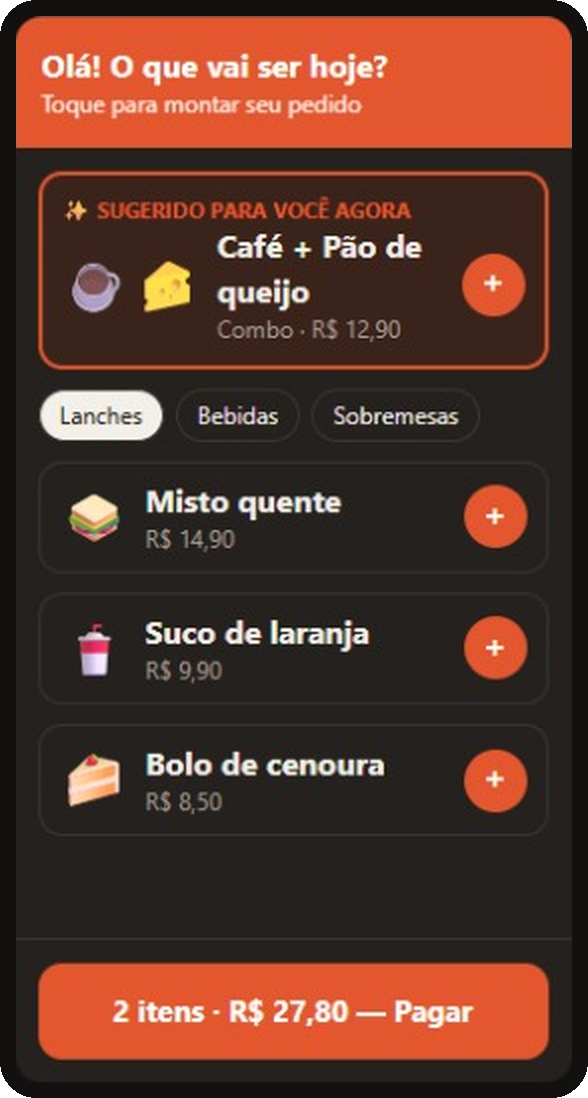
\includegraphics[width=\linewidth]{tela-1-cardapio.png}\\[2pt]
        \small (a) Cardápio
    \end{minipage}\hfill
    \begin{minipage}{0.27\textwidth}
        \centering
        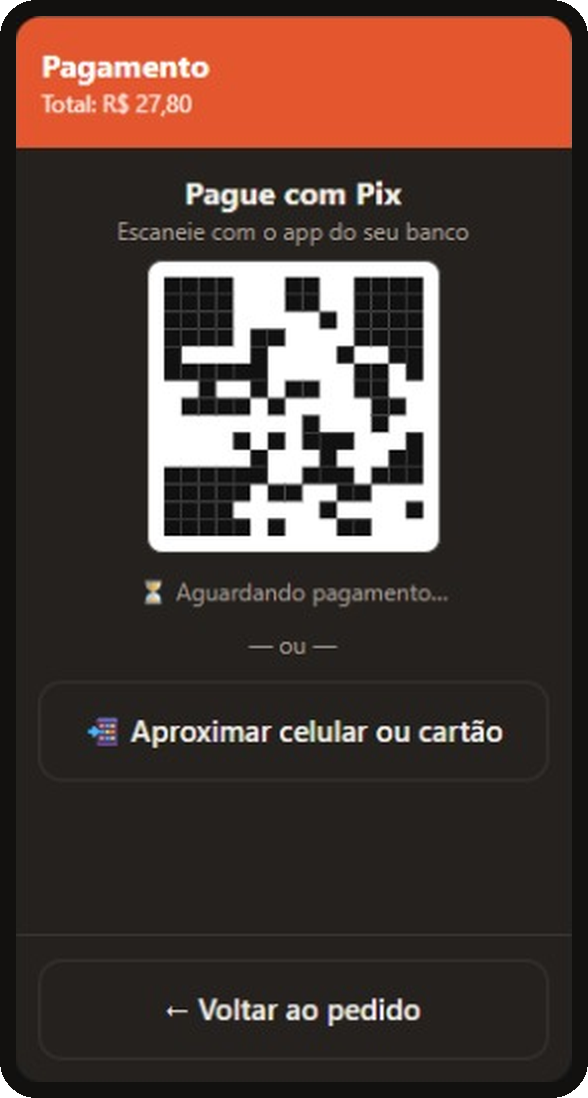
\includegraphics[width=\linewidth]{tela-2-pagamento.png}\\[2pt]
        \small (b) Pagamento
    \end{minipage}\hfill
    \begin{minipage}{0.27\textwidth}
        \centering
        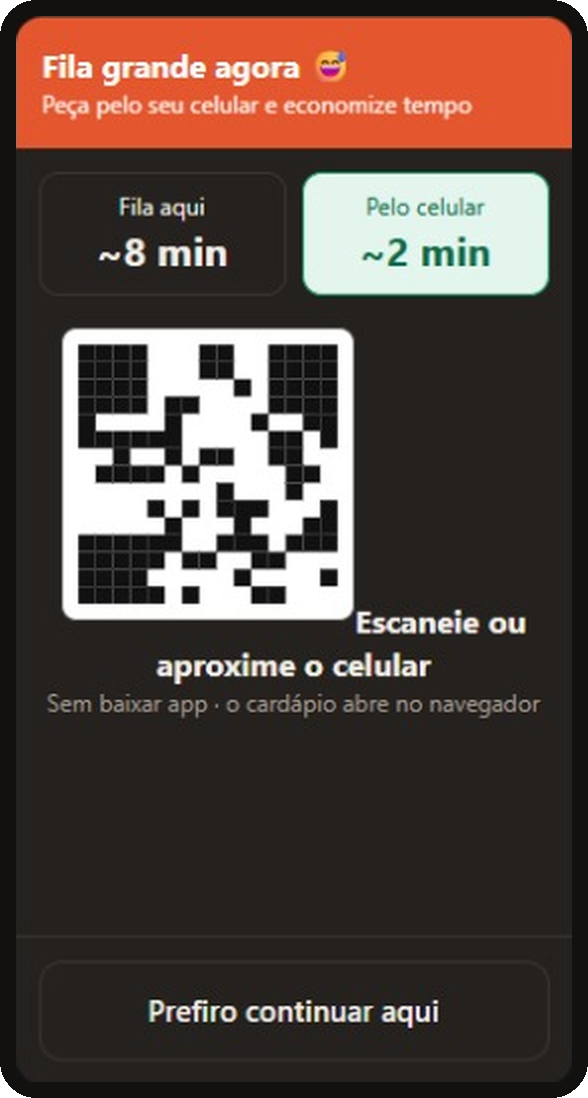
\includegraphics[width=\linewidth]{tela-3-fila-cheia.png}\\[2pt]
        \small (c) Fila cheia
    \end{minipage}
    \caption{Telas do protótipo mostradas aos entrevistados}
    \label{fig:telas}
\end{figure}

\subsection{Tela 1: Cardápio}

\begin{enumerate}
    \item Olhando essa tela, você saberia fazer um pedido sozinho, sem ajuda?
    \item Esse totem \textbf{resolveria} a espera ou o atendimento que você costuma enfrentar nesses lugares? \textit{Escala de 1 (nada) a 5 (totalmente).}
    \item A ``sugestão para você'' ajuda ou incomoda? Como você se sentiria sabendo que ela é feita por uma câmera no aparelho? \textit{Aberta: anotar a reação espontânea sobre privacidade.}
\end{enumerate}

\subsection{Tela 2: Pagamento}

\begin{enumerate}
    \setcounter{enumi}{3}
    \item Você pagaria por aqui em vez de ir ao caixa? Por quê (ou por que não)?
    \item O que te deixaria inseguro ao pagar nesse totem? \textit{Aberta: anotar confiança, medo de erro ou falta de recibo.}
    \item Você \textbf{pagaria} mais caro (ex.: R\$ 1 a mais) por essa comodidade, ou só usaria se fosse igual ao caixa? \textit{Sim, só se igual ou não.}
\end{enumerate}

\subsection{Tela 3: Fila cheia}

\begin{enumerate}
    \setcounter{enumi}{6}
    \item Se a fila estivesse grande, você pediria pelo próprio celular ou esperaria o totem? Por quê?
    \item Escanear ou aproximar o celular sem baixar app é tranquilo para você? O que travaria?
    \item No geral: você \textbf{usaria} esse totem no lugar do caixa? \textit{Escala de 1 a 5; perguntar o motivo da nota.}
\end{enumerate}

\section{Análise}

As respostas são consolidadas por hipótese, somando as 75 entrevistas:

\begin{itemize}
    \item \textbf{Escalas} (perguntas 2 e 9): média e distribuição das notas, com os motivos agrupados por tema.
    \item \textbf{Pergunta fechada} (6): proporção de respostas ``sim'', ``só se igual'' e ``não''.
    \item \textbf{Perguntas abertas}: reações agrupadas por tema, como privacidade da câmera (3), confiança no pagamento (5) e barreiras para usar o QR Code ou o NFC (8).
\end{itemize}

\begin{thebibliography}{99}

\bibitem{fecomercio2026}
FECOMERCIO-SP. \textbf{Custo do trabalho aumentaria 22\% com fim da escala 6x1}. Notícias FecomercioSP, São Paulo, 12 fev. 2026. Disponível em: \url{https://www.fecomercio.com.br/noticia/custo-do-trabalho-aumentaria-22-com-fim-da-escala-6x1}. Acesso em: 16 ago. 2026.

\bibitem{abrasel2026}
ABRASEL - ASSOCIAÇÃO BRASILEIRA DE BARES E RESTAURANTES. \textbf{Fim da escala 6x1: impactos econômicos e operacionais da mudança na jornada no setor de alimentação}. Análise Institucional Abrasel / CNN Brasil, 18 abr. 2026. Disponível em: \url{https://www.cnnbrasil.com.br/economia/macroeconomia/abrasel-fim-da-escala-6x1-avanca-por-interesse-eleitoral-e-de-modo-acodado/}. Acesso em: 16 ago. 2026.

\end{thebibliography}


\end{document}
